\documentclass{beamer}

\usepackage{amsmath, amssymb, hyperref, graphics, wasysym}
\usepackage{mathpazo, tikz}

\newcommand{\C}{\mathbb{C}}
\newcommand{\Z}{\mathbb{Z}}
\newcommand{\R}{\mathbb{R}}
\DeclareMathOperator{\Hom}{\text{Hom}}
\title{MAS439 Lecture 6 \\ Examples of Quotient Rings \\ What's the Universal Property all about?}

\date{October 12th}

\begin{document}

\begin{frame}
\titlepage
\end{frame}

\begin{frame}{Last time, we introduced the quotient ring $R/I$}
  \begin{definition} Let $R$ be a ring, and $I$ an ideal.  Then the ring $R/I$ is the set of equivalence classes of elements of $R$, where $r\sim s$ if $r-s\in I$.

    Addition and multiplication are given by adding and multiplying representatives:
    $$[r]+[s]=[r+s]$$
    $$[r]\cdot [s]=[r\cdot s]$$
    $$1_{R/I}=[1]$$
  \end{definition}

  \begin{lemma}The map $p:R\to R/I$ defined by $p(r)=[r]$ is a homomorphism.
  \end{lemma}
  \end{frame}

\begin{frame}{The problem with this definition:}
  To talk about what the elements are, we need to understand what the equivalence classes are.

  \begin{block}{Usually we want to pick a unique representative from each class}
    This is exactly like thinking:
    $$\Z/n=\{0,1,\dots, n-1\}$$
    instead of the strict definition:
    $$\Z/n=\Big\{\{a+n\Z\} : a\in \Z\Big\}$$
    \end{block}
  \begin{block}{The division algorithm is a good way to do this}
    \end{block}


  \end{frame}



\begin{frame}[plain,c]

\begin{center}

\Huge

\usebeamercolor[fg]{frametitle}
Examples
\end{center}

\end{frame}


\begin{frame}{Example: $\C\cong\R[x]/(x^2+1)$}

\begin{block}{The division algorithm gives unique representatives}

Any polynomial $p(x)$ can be written uniquely as

 $$p(x)=(x^2+1)q(x)+bx+a$$. 

This means that $[p(x)]=[bx+a]$, so every class can be represented by a linear polynomial; furthermore, this representation is unique.
\end{block}

It's clear $[a+bx]+[c+dx]=[a+c+(b+d)x]$.
\end{frame}

\begin{frame}{Example: $\mathbb{C}=\R[x]/(x^2+1)$}

\begin{block}{Multiplication of representatives}
$$[a+bx]\cdot [c+dx]=[ac+(ad+bc)x+bdx^2]$$

But this isn't linear;  we need to get rid of the $x^2$ term.  Note that $bdx^2=bd(x^2+1)-bd$, and so $[bdx^2]=[-bd]$.

Thus, we see
$$[a+bx]\cdot [c+dx]=[ac-bd+(ad+bc)x]$$
which, if we replace $x$ with $i$, is exactly the formula for multiplying complex numbers.
\end{block}


\end{frame}


\begin{frame}{Example: $\R[x]/(x^2)$}

First, we have to understand it as a set -- we want to give a \emph{unique} name to each element of $R/I$.  This is usually done by picking a representative from each coset in some systematic way.

$I$ consists of linear combinations of monomials of degree 2 or bigger.  So every equivalence class contains exactly one linear term $a+bx$.  We see that 

$$[a+bx]\cdot [c+dx]=[ac+adx+bcx+adx^2]=[ac+(ad+bc)x]$$


\end{frame}




\begin{frame}{Constructing $\mathbb{F}_4$}

We claim that $R=\mathbb{F}_2[x]/(x^2+x+1)$ is a field with 4 elements.  

Exactly as in the last two examples, the division algorithm gives every equivalence class has a unique linear representative $a+bx$; now $a,b\in\mathbb{F}_2$, so there are indeed four elements.

We check:
$$[x]\cdot [x+1]=[x^2+x]=[1]$$
So every nonzero element has an inverse, and so $R$ is a field.
\end{frame}

\begin{frame}{A case where the division algorithm doesn't hold:}
\begin{block}{Consider the ring $\Z[x]/(10x-1)$:}
Can't divide $x$ by $10x-1$ and get a polynomial of lower degree.  
\end{block}

\begin{block}{What is this ring, intuitively?}
  Since we're setting $10x-1=0$, then $x$ ``should be'' $1/10$.  So, we've taken the integers and added $1/10$.
  \end{block}

\begin{block}{How to make this intuition formal?}
To really understand the ring $\Z[x]/(10x-1)$, will find two different systems ofunique representatives for the equivalence classes.
\end{block}
  
  \end{frame}


\begin{frame}{Method 1: Muddle along with division algorithm}
  \begin{lemma}
    For any polynomial $p(x)\in\Z[x]$, there is a unique polynomials $q(x)$ and a unique integer $r$, so that
    \begin{itemize}
    \item $p(x)=q(x)(10x-1)+r$
    \item $q(x)=\sum a_n x^n$ with $0\leq a_i\leq 9$
    \end{itemize}
  \end{lemma}

  \begin{proof}
    \begin{itemize}
    \item Existence
    \item Uniqueness
\end{itemize}
    \end{proof}

 Every number in $\Z[1/10]$ has a unique terminating binary expansion.


  \end{frame}

\begin{frame}{Method 2: Divide ``backwards''}

  \begin{lemma} For any $p(x)\in\Z[x]$, there is a unique $q(x)\in\Z[x]$, $n\geq 0$, and $a\in\Z$, so that
    $$p(x)=q(x)(1-10x)+ax^n$$
and $a$ is not divisible by 10 if $n>0$.  
  \end{lemma}
  \begin{proof}
    \begin{itemize}
    \item Existence: divide backwards as power series to get remainder $ax^m$, if $10$ divides $a$, then backtrack
    \item Uniqueness
    \end{itemize}
  \end{proof}

  This is writing an element of $\Z[1/10]$ as $a/10^n$, and then if $a$ is divisible by 10 we can cancel some powers of 2.
    \end{frame}

\begin{frame}[plain,c]

\begin{center}

\Huge 

\usebeamercolor[fg]{frametitle}
The Universal Property of Quotient Rings
\end{center}

\end{frame}

\begin{frame}[fragile]{The Universal Property for Quotient rings}
Suppose that $\varphi:R \to S$ is a ring homomorphism such that $I\subset \ker(\varphi)$, and let $p:R\to R/I$ be the quotient map.   Then there exists a unique ring homomorphism $\overline{\varphi}:R/I\to S$ satisfying $\varphi=\overline{\varphi}\circ p$.

\begin{block}{Put another way}
The following diagram commutes:
\begin{center}
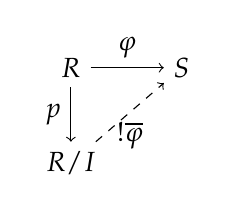
\begin{tikzpicture}[every node/.style={midway}]
\matrix[column sep={4em,between origins},
        row sep={2em}] at (0,0)
{ \node(R)   {$R$}  ;  & \node(S) {$S$}; \\
  \node(R/I) {$R/I$  };                   \\};
\draw[<-] (R/I) -- (R) node[anchor=east]  {$p$};
\draw[->, dashed] (R/I) -- (S) node[anchor=north]  {$ !\overline{\varphi}$};
\draw[->] (R)   -- (S) node[anchor=south] {$\varphi$};
\end{tikzpicture}
\end{center}
\end{block}

\end{frame}

\begin{frame}{What the universal property ``really means''}
\begin{block}{Universal property as a slogan:}
Maps out of $R/I$ are the same thing as maps out of $R$ whose kernel contains $I$
\end{block}

This property \emph{defines} the quotient ring $R/I$.

\begin{lemma} Let $R$ be a ring, and $I$ be an ideal.  If $q:R\to T$ also satisfies the universal property of the quotient ring, then we have $T\cong R/I$.
\end{lemma}

\begin{proof}
 All we have is the Universal Property, so we're going to use it over and over again\dots
  \end{proof}.
Universal properties are an idea from category theory
\end{frame}

\begin{frame}{Definition of a category}
  A category $\mathcal{C}$ consists of
  \begin{itemize}
  \item A collection of objects $Ob(\mathcal{C})$
  \item For every pair of objects $A, B$ a set $\Hom_{\mathcal{C}}(A,B)$ of morphisms (or arrows)
  \end{itemize}
  We write $f:X\to Y$ to mean $f\in \Hom_{\mathcal{C}}(A,B)$.
 
  We can compose arrows that line up (i.e., if $f:X\to Y, g:Y\to Z$ then we can make $gf:X\to Z$)

  This composition is associative; and every object has an identity morphism $1_A$ so that $f1_A=1_Bf=f$.

\end{frame}

\begin{frame}{Examples of categories}
  \begin{itemize}
  \item Sets and functions between them
  \item Groups and group homomorphisms
  \item Rings and ring homomorphisms
  \item Vector spaces over a field $k$ and linear maps between them
  \item Topological spaces and continuous maps between then
  \end{itemize}
  All of the above are examples where our objects are sets, and our morphisms are maps between the sets preserving some kind of structure, but categories don't have to be this way.
\end{frame}

\begin{frame}{Category theory is a philosophy}
  \begin{itemize}
    \item Rather than study an object itself, we should study how it relates to other object of its kinds.
    \item moves the focus to the \emph{morphisms}
    \item Really focus goes farther, between how different categories relate to each other...
    \item Captures when you do the same thing in different categories 
  \end{itemize}
\end{frame}

\begin{frame}[fragile]{Example tying this together: product as a Universal Property}
  \begin{definition}
    Let $X, Y$ be two objects in a category $\mathcal{C}$.  The product, $X\times Y$, is an object of $\mathcal{C}$ together with maps $p_1:X\times Y\to X$ and $p_2:X\times Y\to Y$ satisfying the following universal property: for every object $Z$ and pair of maps $f:Z\to X, g:Z\to Y$, there is a unique map $h$ so that $f=p_1h$ and $g=p_2h$.
  \end{definition}
\begin{center}
      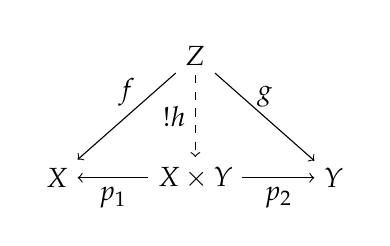
\begin{tikzpicture}[every node/.style={midway}]
\matrix[column sep={5em,between origins},
        row sep={3em}] at (0,0)
{ & \node(Z) {$Z$};  &   \\
 \node(X) {$X$}; &  \node(XY) {$X\times Y$}; & \node(Y) {$Y$};          \\};
\draw[->] (Z) -- (X) node[anchor=south]  {$f$};
\draw[->, dashed] (Z) -- (XY) node[anchor=east]  {$!h$};
\draw[->] (Z)   -- (Y) node[anchor=south] {$g$};
\draw[->] (XY) -- (X) node[anchor=north] {$p_1$};
\draw[->] (XY) -- (Y) node[anchor=north] {$p_2$};

    \end{tikzpicture}
\end{center}

\end{frame}


\end{document}
  
